\section{Rețele neuronale convoluționale (CNNs)}

Motivația din spatele acestor tipuri de rețele a apărut atunci când cercetătorii au încercat să aplice tehnicile clasice de deep learning în domeniul computer vision. Cel mai mare impediment a fost lipsa puterii computaționale. Spre exemplu, pentru o imagine RGB cu dimensiunile $32x32x3$ avem un vector de intrare cu $3072$ de componente, iar dacă primul layer din rețea are $3500$ de neuroni, prima matrice de parametri va avea forma $3500x3072$, adică peste 10 milioane de parametrii de optimizat numai pentru primul layer. Este evident faptul că, pentru ca deep learning să fie aplicat în recunoașterea imaginilor, ne trebuie o altă abordare.

\subsection{Operația de convoluție}
Fie 2 matrici, $I$ matricea de pixeli corespunzătoare unei imagini și $K$ o matrice $kernel (filter)$. Operația de convoluție având ca termeni $I$ și $K$ arată în felul următor:

\begin{center}
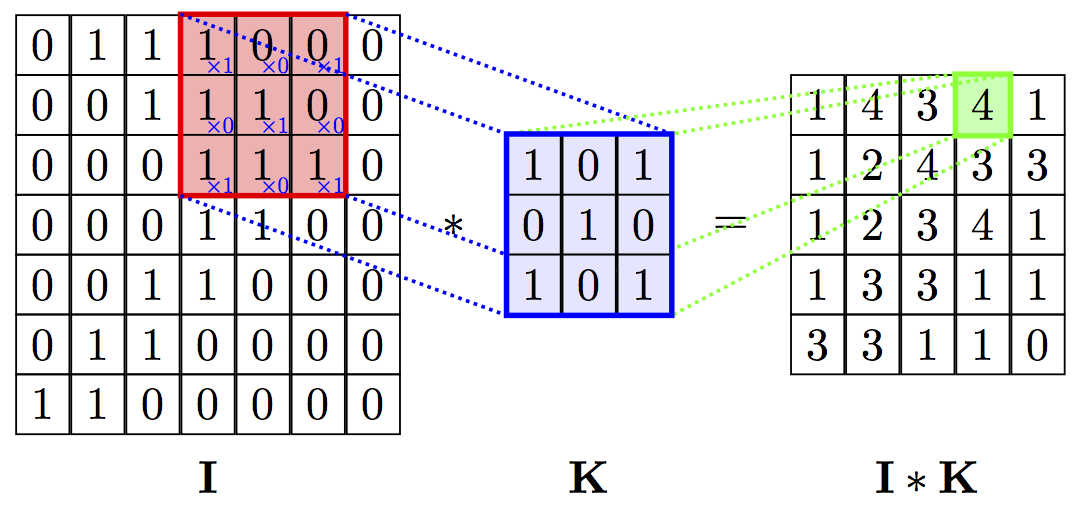
\includegraphics[scale=1.5]{convolution} \\
\textit{Fie I de forma (n,n) și K de forma (f,f). Matricea rezultat va avea forma (n-f+1,n-f+1)}
\end{center}


\subsubsection{Padding și Striding}
Padging-ul a venit ca o soluție pentru cazul în care filter-ul iese în afara imaginii în aproprierea marginilor acesteia. Astfel se va completa matricea inițială cu zero-uri înaintea efectuării operației propriu-zise.

\begin{center}
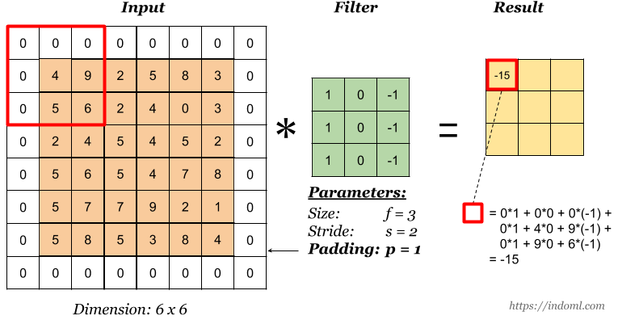
\includegraphics[scale=0.7]{padding}
\end{center}

Această tehnică modifică regula dimensiunii output-ului. Pentru un padding de dimensiune $p$ vom aveaun output de forma $(n+2p-f+1, n+2p-f+1)$. Observăm că operația de convoluție clasică (fără padding) micsorează imaginea, însă, dacă vrem să evitam acest lucru, putem alege un padding $\displaystyle{p=\frac{f-1}{2}}$.

Stridding-ul se referă la numărul de unități cu care vom mișca filter-ul pantru a scana întreaga imagine. Până acum am folosit un stride $s=1$.

\begin{center}
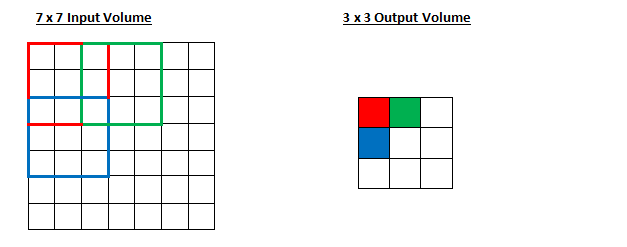
\includegraphics[scale=1]{stride} \\
\textit{Operație de convoluție cu stride-ul s = 2}
\end{center}

Scopul acestei tehnici este să reducă numărul de operații având ca compromis, o mică pierdere de informație. Astfel output-ul obținut va avea forma $\displaystyle{\left(\displaystyle{\left[\frac{n+2p-f}{s}\right]}+1, \displaystyle{\left[\frac{n+2p-f}{s}\right]}+1\right)}$.

\subsubsection{Convoluție peste volume}

Deocamdată, am vorbit despre operația de convoluție pe matrici de pixeli de forma $(n,m)$ ce reprezintă imagini $greyscale$. în contextul imaginilor RGB, matricile lor au forma $(n,m,3)$, iar pentru a putea efectua operația, vom copia filter-ul de 3 ori, formând o matrice de forma $(f,f,3)$. Pentru fiecare channel, vom lua filter-ul si vom face calculele ca înainte, obtinând 3 numere pentru fiecare poziție din output. La final vom aduna aceste 3 numere pentru a calcula o componentă a output-ului, forma acestuia rămânând aceeași ca în cazul imaginilor cu un singur channel.

\begin{center}
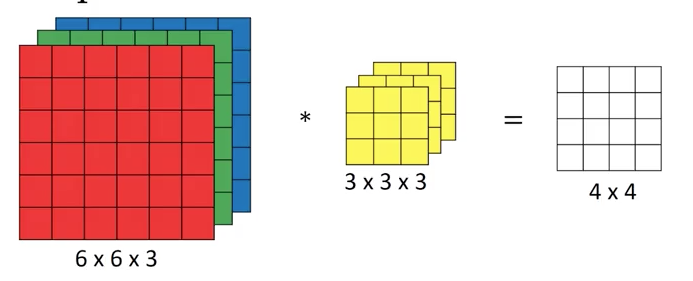
\includegraphics[scale=0.4]{convVolumes} \\
\end{center}

După ce am studiat ce este un filter și operația de convoluție, putem defini un layer într-o rețea neuronală convoluțională ca o multitudine de filtere și de operații de convoluție efectuate pe o matrice de pixeli. Aceste operații sunt independente, însă output-ul lor este combinat la final în următorul mod:

\begin{center}
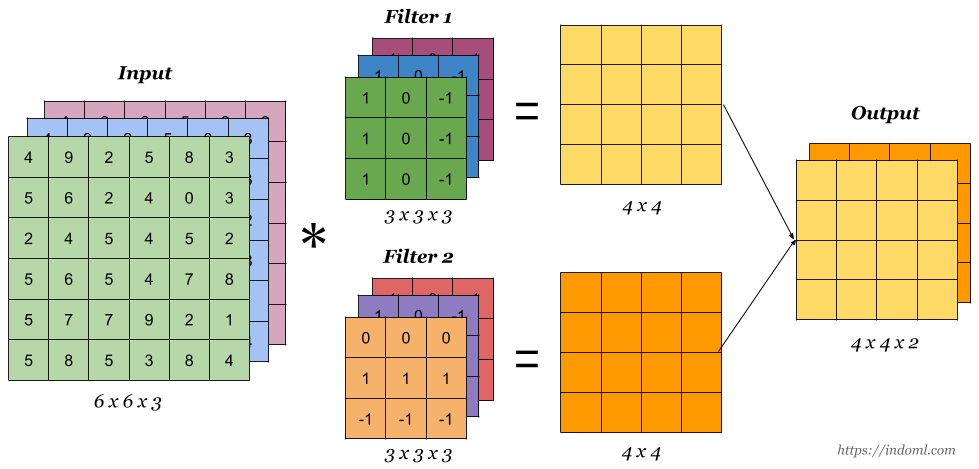
\includegraphics[scale=0.4]{convLayer} \\
\textit{Un layer cu 2 filtere}
\end{center}

Vom compara această abordare cu cea a rețelelor neuronale clasice. Având 2 filtere, vom lua cazul clasic a unui layer cu 2 neuroni obișnuiți. În contextul clasic, având un input de forma $(6,6,3)$ și 2 neuroni, matricea de parametrii va avea forma $(2,6*6*3)$, în total 216 de parametrii. În cazul rețelelor convoluționale, avem 2 filtere de forma $(3,3,3)$, în total 54 de parametrii, făcând aceste rețele mult mai viabile pentru prelucrarea imaginilor de rezoluție înaltă.

\subsection{Arhitecturi celebre}

\subsubsection{LeNet-5}

\subsubsection{VGG-16}

\subsubsection{ResNet}

\subsubsection{Inception}

\subsubsection{Xception}

